\documentclass[10pt,twocolumn]{article}
\usepackage[T1]{fontenc}
\usepackage[utf8]{inputenc}
\usepackage[margin=0.66in]{geometry}
\usepackage{amsmath,amssymb}
\usepackage{booktabs}
\usepackage{pifont}
\usepackage{float}
\usepackage{flafter}
\usepackage{microtype}
\usepackage{xcolor}
\usepackage{graphicx}
\usepackage[colorlinks=true,linkcolor=blue,citecolor=blue,urlcolor=blue]{hyperref}
\usepackage{authblk}
\usepackage[inline]{enumitem}
\setlist{topsep=2pt,itemsep=0pt,parsep=0pt,partopsep=0pt,leftmargin=*}

% let LaTeX pack floats more tightly than the article defaults allow
\setcounter{topnumber}{3}\setcounter{bottomnumber}{2}\setcounter{totalnumber}{4}
\setcounter{dbltopnumber}{3}
\renewcommand{\topfraction}{0.92}\renewcommand{\bottomfraction}{0.5}
\renewcommand{\textfraction}{0.06}\renewcommand{\floatpagefraction}{0.80}
\renewcommand{\dbltopfraction}{0.92}\renewcommand{\dblfloatpagefraction}{0.80}

% Tables generated OUTSIDE this directory (tables/replication.tex, written by
% bench/exp_causal_replication.py) do not set their own column separation, and a
% \setlength inside a group would not survive to float-output time.  So the document
% default is set narrow here; every locally generated table overrides it in its own body.
\setlength{\tabcolsep}{2.6pt}

\graphicspath{{figures/}}
\newcommand{\cafe}{CAF\'E}
% robust: \nobreakdash is fragile inside captions (moving arguments)
\DeclareRobustCommand{\cd}{\cafe{}\nobreakdash-CD}

\title{\textbf{\cd{}: Point-in-Time Causal Discovery on
Factor-Adjusted Residuals}\\[3pt]
  {\large\normalfont A short results paper --- where factor residualisation wins,
  where it loses and why, what three public benchmarks are actually measuring, and
  what a causality certificate costs}}
\author[1]{Derek Snow}
\author[1]{Matthew Lyberg}
\author[1]{Eeshaan Asodekar}
\affil[1]{Sovai Research \quad \texttt{d.snow@sov.ai}}
\date{}

%% generated by experimental/papers/causal/scripts/make_tables.py
\newcommand{\HHrank}{1 of 15}
\newcommand{\HHnbase}{14}
\newcommand{\HHchiA}{0.50}
\newcommand{\HHchiB}{0.95}
\newcommand{\HHcafeA}{0.985}
\newcommand{\HHcafeB}{0.929}
\newcommand{\HHbestLo}{0.708}
\newcommand{\HHbestHi}{0.720}
\newcommand{\HHgapLo}{0.219}
\newcommand{\HHgapHi}{0.267}
\newcommand{\HHgapA}{0.265}
\newcommand{\HHresLo}{-0.048}
\newcommand{\HHresHi}{+0.086}
\newcommand{\HHresMu}{+0.011}
\newcommand{\HHrtCafe}{4.01}
\newcommand{\RTcafe}{2.42}
\newcommand{\RTpcmci}{49.55}
\newcommand{\RTspeed}{21}
\newcommand{\RTnz}{0.917}
\newcommand{\RTnart}{52}
\newcommand{\RTbeats}{13}
\newcommand{\RTrtAuc}{0.921}
\newcommand{\RTrtTrans}{0.554}
\newcommand{\RTspeedSmall}{3.6}
\newcommand{\RTsmallN}{5}
\newcommand{\RTsmallT}{300}
\newcommand{\DGn}{40}
\newcommand{\DGrep}{0.278}
\newcommand{\DGcond}{0.055}
\newcommand{\DGcondRaw}{0.077}
\newcommand{\DGwRep}{38/40}
\newcommand{\DGwRawBiv}{34/40}
\newcommand{\DGwResBiv}{23/40}
\newcommand{\DGrawCond}{0.771}
\newcommand{\DGresCond}{0.493}
\newcommand{\DGresBiv}{0.548}
\newcommand{\DGrawBiv}{0.848}
\newcommand{\DGcafe}{0.541}
\newcommand{\DGcafeFone}{0.443}
\newcommand{\DGmarg}{0.616}
\newcommand{\DGtol}{0.46}
\newcommand{\DGwbiv}{0.40}
\newcommand{\DGrank}{3.5}
\newcommand{\DGmc}{0.746}
\newcommand{\DGxc}{0.932}
\newcommand{\DGcn}{63.9}
\newcommand{\DGle}{0.800}
\newcommand{\SCn}{25}
\newcommand{\SConLo}{13}
\newcommand{\SConHi}{74}
\newcommand{\SCoffHi}{1.45}
\newcommand{\SCsdOff}{0.375}
\newcommand{\SCnneg}{14}
\newcommand{\SCnnegz}{4}
\newcommand{\SCshz}{0.041}
\newcommand{\SCsdLo}{0.030}
\newcommand{\SCsdHi}{175.5}
\newcommand{\SCvsRaw}{0.99}
\newcommand{\SCvsRes}{0.76}
\newcommand{\SCrsRaw}{0.30}
\newcommand{\SCrsRes}{0.33}
\newcommand{\SPngain}{5}
\newcommand{\SPnflat}{7}
\newcommand{\SPglo}{+0.2448}
\newcommand{\SPghi}{+0.3085}
\newcommand{\SPcafe}{-0.1012}
\newcommand{\SPcafeScale}{0.4524}
\newcommand{\SPcafeFree}{0.5536}
\newcommand{\SPn}{150}
\newcommand{\CRFloodScaleRank}{11}
\newcommand{\CRFloodScaleN}{14}
\newcommand{\CRFloodScaleCafe}{0.257}
\newcommand{\CRFloodScaleTop}{DYNOTEARS}
\newcommand{\CRFloodScaleTopAP}{0.625}
\newcommand{\CRFloodScaleVar}{0.614}
\newcommand{\CRFloodFreeRank}{4}
\newcommand{\CRFloodFreeN}{14}
\newcommand{\CRFloodFreeCafe}{0.345}
\newcommand{\CRFloodFreeTop}{Granger (pairwise)}
\newcommand{\CRFloodFreeTopAP}{0.472}
\newcommand{\CRFloodFreeVar}{0.416}
\newcommand{\CREastConfRank}{6}
\newcommand{\CREastConfN}{13}
\newcommand{\CREastConfCafe}{0.565}
\newcommand{\CREastConfTop}{DirectLiNGAM}
\newcommand{\CREastConfTopAP}{0.731}
\newcommand{\CREastConfVar}{0.696}
\newcommand{\CREastRandRank}{8}
\newcommand{\CREastRandN}{13}
\newcommand{\CREastRandCafe}{0.549}
\newcommand{\CREastRandTop}{VAR-OLS}
\newcommand{\CREastRandTopAP}{0.792}
\newcommand{\CREastRandVar}{0.792}
\newcommand{\DYrank}{6}
\newcommand{\DYn}{54}
\newcommand{\DYcafe}{0.729}
\newcommand{\DYtop}{PCMCI$+$}
\newcommand{\DYtopAP}{0.800}
\newcommand{\DYnbelow}{10}
\newcommand{\DYnmeth}{13}
\newcommand{\DYfloor}{0.759}
\newcommand{\LossVarCount}{5}
\newcommand{\LossCfgCount}{5}
\newcommand{\LossVarAll}{all 5}
\newcommand{\MatchCoupled}{7}
\newcommand{\BaseCoupled}{10}
\newcommand{\CafeCoupled}{132}
\newcommand{\MatchClimate}{11}
\newcommand{\BaseClimate}{12}
\newcommand{\CafeClimate}{12}

\begin{document}
\maketitle

\begin{abstract}
\noindent
\cd{} runs causal discovery on the idiosyncratic residuals of a strictly
point-in-time dynamic factor model: \cafe{} residualisation, engine routing,
backward-only lag screening, a panel group-lasso skeleton, and assumption-routed
orientation with explicit abstention. It is numpy-only and CPU-only; every stage reads
rows $\le t$, so the graph reported at $t$ is truncation-invariant by construction. This
paper reports what we measured, including the parts that do not favour us.
\textbf{(1)~We win decisively on panel data.} On synthetic panels whose ground truth we
audit ourselves, \cd{} is rank \HHrank{} at every common-variance share $\chi$ ---
$\HHcafeA$ at $\chi{=}\HHchiA$ down to $\HHcafeB$ at $\chi{=}\HHchiB$, against a best
baseline that never leaves $\HHbestLo$--$\HHbestHi$. A fairness arm re-runs every
baseline on the \emph{identical} \cafe{} residual and moves it by $\HHresLo$ to
$\HHresHi$, so the margin is the discovery machinery, not the preprocessing. The baselines
are single-series methods applied per entity: pooling the entity dimension is a real
advantage and it is most of what the table measures.
\textbf{(2)~We lose on single-series benchmarks, and we measured why.} On the published
CausalRivers cell \cd{} ranks $\CRFloodScaleRank$ of $\CRFloodScaleN$, behind a
$1$\,ms OLS VAR. Holding the estimator
and the moment tensor fixed and varying only two design choices decomposes the loss:
residualising costs $\DGrep$ AUROC and conditioning on every other source rather than
one costs a further $\DGcond$. Part of that first term is a \textbf{located library
defect}: \cafe{}'s ARD rank selection is not scale-equivariant, so below unit scale the
factor adjustment removes \emph{nothing}, and on unrescaled river discharge it is
mis-scaled rather than merely idle. We report it with its measured cost and its
re-certification requirement, not as a pending win --- no benchmark verdict changes. A
second limit, measured on our own generator, is that the evidence blend's premium over
its best single component is monotone in the number of entities and turns
\emph{negative} at $E{=}1$ --- and every public single-series benchmark is $E{=}1$. We
deliberately shipped no gate for it: the effect is a hundredth of an AUC and fitting one
would be the benchmark-fitting we criticise. Three further hypotheses were tested and
falsified, and are reported.
\textbf{(3)~Benchmark forensics.} We reproduce five published CausalRivers cells, then
show the same VAR moves $0.849\to0.593$ on all 2\,139 subgraphs by switching to a
scale-free statistic; the true graphs have var-sortability $0.939$. We reproduce the
CausalDynamics \texttt{coupled} leaderboard from the authors' own shipped artefacts, and
then find that a \emph{constant identity matrix} scores $0.682/0.353$ there and no
shipped method beats it. Two \texttt{simple} cells are broken and we reproduce both
published AUROCs to $10^{-3}$ by replicating the defect; a third defect feeds an
endpoint matrix to a ranking metric.
\textbf{(4)~A point-in-time board}, now complete: every published method is batch, and
churn and a leakage delta on each method's own metric say what that costs.
\textbf{(5)~Runtime}: $\RTspeed\times$ faster than PCMCI$+$ on a real 12-variable
series at the same dense submission. Limitations get their own section.
\end{abstract}

\section{The method}\label{sec:method}
\cd{} is the discovery read-out of \cafe{}~\cite{cafe}, a causal (strictly
point-in-time) dynamic factor model whose forward pass already produces imputations,
factors and residuals. The pipeline is five stages behind one public call,
\texttt{cafe.discover(df)}:

\begin{enumerate}
\item \textbf{Residualise.} Take the factor-adjusted residual of the causal one-pass
  model. A latent common factor is a textbook confounder, so it is projected out by the
  same point-in-time pass that did the imputation. The residual is deliberately
  \emph{not} winsorised: the tail is exactly what identifies edge direction in every
  LiNGAM-family branch downstream~\cite{shimizu2006,hyvarinen2010}.
\item \textbf{Route the loading engine} (panels only), \S\ref{sec:eng}.
\item \textbf{Screen lags} with a backward-only sign-correlation statistic whose
  threshold comes from a circular-block permutation null, not a constant. The encoding
  reads only indices $\le t$; a forward-looking control is asserted to fail that test.
\item \textbf{Skeleton.} A panel group lasso on the surviving candidates fits a shared
  $B_0$ plus sparse per-entity deviations and selects the support.
\item \textbf{Orient.} Lagged edges are oriented by the arrow of time for free; only
  the contemporaneous ambiguous graph is searched, per connected component. The
  orienter \emph{abstains} --- emitting \texttt{o-o} or \texttt{<->} --- when no
  branch's assumptions hold, rather than manufacturing a DAG.
\end{enumerate}

\noindent
\texttt{mode="pit"} truncates the panel and runs the identical pipeline, so the
reported graph is truncation-invariant by construction. Dependencies: numpy.

\section{Scope, stated up front}\label{sec:gate}
The obvious objection to residualising before discovery is that it can only help if
there is a factor worth removing. That is right, and the interesting question is where
the boundary sits. We generate panels with a tunable common-variance share $\chi$ and
feed three \emph{identical} representations --- raw, \cd{} residual, oracle residual
(true factors removed) --- to three downstream estimators. The sparse estimators are
scored threshold-free by lambda entry order, so no model-selection rule enters
anywhere. Table~\ref{tab:gate} and Figure~\ref{fig:gate} are the result.

\begin{figure}[t]
\centering
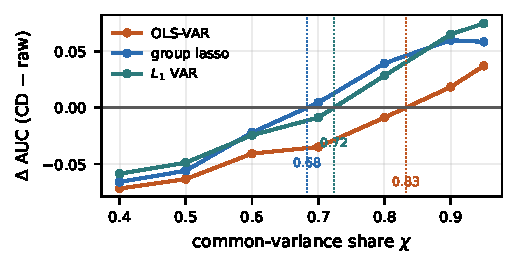
\includegraphics[width=\columnwidth]{gate.pdf}
\caption{The crossover: paired advantage of the \cafe{}-CD residual over raw against
$\chi$, dotted lines at $\chi^\star$. The effect is a shallower decline, not a higher
ceiling; Table~\ref{tab:gate} has the levels.}
\label{fig:gate}
\end{figure}

% generated by experimental/papers/causal/scripts/make_tables.py
% source: bench/causal_sparse_gate_cache.base.json
\begin{table*}[t]\centering\small
\setlength{\tabcolsep}{3.2pt}
\caption{\textbf{Factor residualisation helps only above a crossover in the
common-variance share $\chi$, and a \emph{sparse} downstream estimator moves that
crossover down.} Off-diagonal lagged-edge AUC for identical representations fed to
three downstream estimators: \textsc{raw} the observed panel, \textsc{cd} the \cafe{}
idiosyncratic residual, \textsc{orc} the oracle residual (true factors removed). The
sparse estimators are scored threshold-free by lambda entry order, so no model-selection
rule enters. $\Delta$ is the paired mean $(\textsc{cd}-\textsc{raw})$ over 8
seeds, \emph{w} the paired win count, $p$ an exact one-sided sign-flip permutation test,
$\chi^\star$ the interpolated crossover. Panel: $E{=}10$, $T{=}60$, $P{=}24$,
$n/\mathrm{col}{=}12.1$.}
\label{tab:gate}
\begin{tabular}{r|rrrr@{\ }l|rrrr@{\ }l|rrrr@{\ }l}
\toprule
 & \multicolumn{5}{c}{OLS-VAR (unpenalised)} & \multicolumn{5}{c}{panel group lasso} & \multicolumn{5}{c}{$L_1$ VAR (per target)} \\
$\chi$ & raw & \textsc{cd} & orc & $\Delta$ & w/$p$ & raw & \textsc{cd} & orc & $\Delta$ & w/$p$ & raw & \textsc{cd} & orc & $\Delta$ & w/$p$ \\
\midrule
0.40 & 0.979 & 0.907 & 0.992 & -0.072 & 0/1.000 & 0.941 & 0.875 & 0.966 & -0.066 & 0/1.000 & 0.982 & 0.923 & 0.995 & -0.059 & 0/1.000 \\
0.50 & 0.971 & 0.907 & 0.992 & -0.063 & 0/1.000 & 0.922 & 0.866 & 0.966 & -0.056 & 0/1.000 & 0.971 & 0.922 & 0.995 & -0.049 & 0/1.000 \\
0.60 & 0.958 & 0.917 & 0.992 & -0.041 & 0/1.000 & 0.893 & 0.871 & 0.966 & -0.022 & 1/0.996 & 0.951 & 0.927 & 0.995 & -0.024 & 1/0.992 \\
0.70 & 0.938 & 0.903 & 0.992 & -0.035 & 0/1.000 & 0.852 & \textbf{0.856} & 0.966 & +0.005 & 6/0.336 & 0.919 & 0.911 & 0.995 & -0.009 & 2/0.727 \\
0.80 & 0.906 & 0.897 & 0.992 & -0.009 & 2/0.953 & 0.798 & \textbf{0.838} & 0.966 & +0.039 & 8/0.004 & 0.871 & \textbf{0.900} & 0.995 & +0.028 & 8/0.004 \\
0.90 & 0.835 & \textbf{0.854} & 0.992 & +0.018 & 7/0.008 & 0.717 & \textbf{0.777} & 0.966 & +0.060 & 8/0.004 & 0.782 & \textbf{0.847} & 0.995 & +0.065 & 8/0.004 \\
0.95 & 0.753 & \textbf{0.790} & 0.992 & +0.037 & 7/0.008 & 0.643 & \textbf{0.701} & 0.966 & +0.058 & 8/0.004 & 0.692 & \textbf{0.767} & 0.995 & +0.075 & 8/0.004 \\
\cmidrule{2-16}
\multicolumn{1}{r|}{crossover} & \multicolumn{5}{c}{$\chi^\star=0.83$} & \multicolumn{5}{c}{$\chi^\star=0.68$} & \multicolumn{5}{c}{$\chi^\star=0.72$} \\
\bottomrule
\end{tabular}
\end{table*}


\paragraph{The crossover depends on the estimator, and that is the point.} Under an
unpenalised OLS-VAR the crossover is $\chi^\star{=}0.83$; under the panel group lasso
it drops to $0.68$ and under a per-target $L_1$ VAR to $0.72$. This is exactly the
mechanism identified by the factor-adjusted network literature --- FNETS~\cite{fnets}
and Krampe~\cite{krampe} --- made quantitative. A pervasive factor makes the
\emph{observed} VAR dense: every series loads on the factor, so every series
Granger-causes every other. Density is not a problem for unpenalised OLS, which simply
absorbs the factor because it is spanned by its own lagged regressors. It is fatal for
a \emph{sparse} estimator, whose entire premise is that the true transition matrix has
few non-zeros. Removing the factor is therefore worth roughly $15$ points of $\chi$ to
a sparse estimator and nothing to a dense one. At $\chi{=}0.90$ the group lasso gains
$\Delta{=}+0.060$ with 8/8 paired wins and $p{=}0.004$; at $\chi{=}0.40$ it
\emph{loses} $0.066$.

\paragraph{Below the crossover the \emph{representation} is worse than raw.} There is
no way to read Table~\ref{tab:gate} that hides this and we do not try. The routing rule
is structural, not outcome-based (\S\ref{sec:eng}), so it cannot rescue a panel whose
$\chi$ is low --- and it should not: at low $\chi$ the estimated factor is mostly
estimation error, and subtracting it destroys signal. \textbf{But this is a statement
about the representation in isolation, not about the pipeline}, and
\S\ref{sec:h2h} is where the two come apart: the full \cd{} pipeline wins at
$\chi{=}\HHchiA$ by $\HHgapA$ AUC even though residualisation \emph{alone} costs
$0.056$ there. Table~\ref{tab:gate} fixes the downstream estimator and varies the input;
Table~\ref{tab:h2h} varies the whole method. They are answering different questions and
they do not contradict.

\section{Head-to-head on ground truth we audit}\label{sec:h2h}
The benchmarks in \S\ref{sec:forensics} turn out to measure things other than
conditional-independence discovery, so the load-bearing comparison is the one where we
control the data-generating process and can inspect the truth. We generate panels from
\texttt{bench/gen\_causal\_panel.py} --- $E{=}10$ entities, $T{=}120$, $P{=}24$,
rank-3 common component, $K{=}2$ true lags, heterogeneous coefficients, Laplace shocks
--- sweep $\chi$, and run \HHnbase{} baseline configurations against \cd{}.
Table~\ref{tab:h2h} is the result: \textbf{rank \HHrank{} at every $\chi$},
$\HHcafeA$ at $\chi{=}\HHchiA$ falling only to $\HHcafeB$ at $\chi{=}\HHchiB$, against
a best baseline that never leaves $\HHbestLo$--$\HHbestHi$.

% generated by experimental/papers/causal/scripts/make_tables.py
% source: bench/causal_synthetic_h2h_cache.json
\begin{table*}[t]\centering\small
\setlength{\tabcolsep}{4pt}
\caption{\textbf{Head-to-head on ground truth we audit ourselves: \cd{} is rank 1 of
15 at every $\chi$, and the margin survives the fairness arm.} Off-diagonal
lagged-edge AUC (\texttt{auc\_cross}) on panels from \texttt{bench/gen\_causal\_panel.py}
($E{=}10$, $T{=}120$, $P{=}24$, $K{=}2$, Laplace shocks, heterogeneous
$\beta$), 4 seeds per cell. \textbf{The baselines are single-series methods,
applied per entity and averaged --- so \cd{}'s ability to pool $E$ entities is a real
advantage, and it is most of what this table measures.} The \textsc{+res} column
controls for the other half: each baseline re-run on the \emph{identical} \cafe{}
residual, which isolates the discovery machinery from the preprocessing. Across all
28 (method, $\chi$) pairs residualisation moves a baseline by
$-0.048$ to $+0.086$ (mean $+0.011$; it helps 17 of 28), so
the gap to \cd{} is the machinery, not the representation. Runtime is mean seconds per
cell on one CPU.}
\label{tab:h2h}
\begin{tabular}{@{}lrrrrrrrrr@{}}
\toprule
 & \multicolumn{2}{c}{$\chi=0.50$} & \multicolumn{2}{c}{$\chi=0.70$} & \multicolumn{2}{c}{$\chi=0.90$} & \multicolumn{2}{c}{$\chi=0.95$} & \\
method & own & \textsc{+res} & own & \textsc{+res} & own & \textsc{+res} & own & \textsc{+res} & s/cell \\
\midrule
\textbf{\cafe{}-CD} & \textbf{0.985} & --- & \textbf{0.980} & --- & \textbf{0.952} & --- & \textbf{0.929} & --- & 4.01 \\
\midrule
DYNOTEARS & 0.720 & 0.703 & 0.712 & 0.686 & 0.708 & 0.666 & 0.709 & 0.662 & 68.52 \\
VAR-OLS & 0.685 & 0.653 & 0.663 & 0.649 & 0.614 & 0.623 & 0.578 & 0.604 & 0.00 \\
PCMCI & 0.662 & 0.674 & 0.636 & 0.648 & 0.569 & 0.597 & 0.551 & 0.562 & 29.98 \\
Granger (pairwise) & 0.607 & 0.675 & 0.556 & 0.642 & 0.531 & 0.585 & 0.527 & 0.557 & 0.78 \\
PC (lag-augmented) & 0.614 & 0.624 & 0.559 & 0.588 & 0.513 & 0.555 & 0.500 & 0.541 & 122.91 \\
DAGMA (linear) & 0.500 & 0.500 & 0.500 & 0.500 & 0.500 & 0.500 & 0.500 & 0.500 & 17.35 \\
VARLiNGAM & 0.490 & 0.510 & 0.470 & 0.494 & 0.481 & 0.484 & 0.478 & 0.471 & 10.93 \\
\midrule
\multicolumn{1}{@{}l}{\cd{} rank} & \multicolumn{2}{c}{1/15} & \multicolumn{2}{c}{1/15} & \multicolumn{2}{c}{1/15} & \multicolumn{2}{c}{1/15} & \\
\bottomrule
\end{tabular}
\end{table*}


\paragraph{Two things a reader would rightly ask, answered in the table itself.}
First, \textbf{is the margin just the preprocessing?} Every baseline is also run on the
\emph{identical} \cafe{} residual (the \textsc{+res} column). If residualisation were
doing the work, that arm would close the gap. It moves the baselines by $\HHresLo$ to
$\HHresHi$ --- mean $\HHresMu$ --- against a gap of $\HHgapLo$--$\HHgapHi$. It helps
some and hurts others in the pattern \S\ref{sec:gate} predicts rather than lifting
everything: DYNOTEARS, already dense, is \emph{worse} on the residual at every $\chi$,
while VAR-OLS crosses over and is better at high $\chi$. The margin is the discovery
machinery, not the input.

Second, \textbf{is the comparison fair?} Not in the sense of like-for-like
architectures, and we would rather name that than let a reader find it. \cd{} is a
panel method: it pools $E$ entities into one shared skeleton with sparse per-entity
deviations. The baselines are single-series methods; they are applied per entity and
averaged, because that is what they can do. So a large part of what
Table~\ref{tab:h2h} measures is the value of the entity dimension. That \emph{is} the
contribution --- a $T{=}120$, $P{=}24$ single series is hopeless and ten of them are
not --- but it is a claim about panels, and it does not transfer to the single-series
benchmarks in \S\ref{sec:losses}, where it does not.

\section{Benchmark forensics}\label{sec:forensics}
Before claiming anything on a public benchmark we reproduced it, and every criticism
below is earned by a reproduction printed next to it. Our harness matches
five published CausalRivers~\cite{causalrivers} cells across three graph sets and two
metrics (Table~\ref{tab:rivers}a); DYNOTEARS --- re-implemented from the
paper~\cite{dynotears}, since \texttt{causalnex} does not install on Python 3.13 ---
and VARLiNGAM both land \emph{above} the published figures.

% generated by experimental/papers/causal/scripts/make_tables.py
% source: bench/bench_rivers_cache.json
\begin{table}[t]\centering\footnotesize
\setlength{\tabcolsep}{3pt}
\caption{\textbf{(a) Our harness reproduces five published CausalRivers cells}, so
(b) can be read as a statement about the benchmark rather than about our
implementation. $^{\ddagger}$DYNOTEARS is re-implemented from Pamfil et al.\ (2020)
because \texttt{causalnex} does not install on Python 3.13; it and VARLiNGAM land
\emph{above} the published figures. \textbf{(b) The leaderboard is substantially
var-sortability.} The identical VAR on all 2139 flood/Random-5 subgraphs, changing only
the scale convention and the edge statistic --- then the prior measured directly on the
true graphs, with no model fitted. Varsortability is the fraction of true directed edges
whose effect has the larger marginal variance ($0.5$ = no signal, $1$ = sorting by
variance \emph{is} the causal order); $R^2$-sortability is its scale-invariant
counterpart, so standardising does not remove it.}
\label{tab:rivers}
\begin{tabular}{@{}llccrr@{}}
\multicolumn{6}{@{}l}{\textbf{(a) reproduction of published cells}}\\
\toprule
method & cell & metric & $n$ & ours & pub. \\
\midrule
VAR & flood/R-5, Fig.~3a & AUROC & 2139 & 0.8493 & 0.85 \\
VAR & east/R-3, Tab.~3 & AUROC & 1196 & 0.8229 & 0.82 \\
VAR & east/R-3, Tab.~7 & max-$F_1$ & 1196 & 0.8292 & 0.83 \\
DYNOTEARS$^{\ddagger}$ & flood/R-5 & AUROC & 2139 & 0.8157 & 0.79 \\
VARLiNGAM & flood/R-5 & AUROC & 2139 & 0.7400 & 0.72 \\
\bottomrule
\end{tabular}

\vspace{4pt}
\begin{tabular}{@{}lcrr@{}}
\multicolumn{4}{@{}l}{\textbf{(b) four scale conventions, then the prior itself}}\\
\toprule
scoring convention & scale prior & AUROC & max-$F_1$ \\
\midrule
$|\hat\beta|$, unrescaled \emph{(published cell)} & \ding{51} & 0.8493 & 0.6797 \\
$|t|$, unrescaled \emph{(scale-free)} & \ding{55} & 0.5931 & 0.5154 \\
$|\hat\beta|$, benchmark min--max rescale & \ding{55} & 0.4773 & 0.4423 \\
$|\hat\beta|$, wrapper $z$-score & \ding{55} & 0.4256 & 0.4256 \\
\midrule
varsortability of the true graphs & --- & \textbf{0.9393} & sd\,0.110 \\
$R^2$-sortability of the true graphs & --- & 0.3762 & sd\,0.254 \\
\bottomrule
\end{tabular}
\end{table}

%% generated by experimental/papers/causal/scripts/make_tables.py
\begin{table*}[t]
\begin{minipage}[t]{0.485\textwidth}% generated by experimental/papers/causal/scripts/make_tables.py
% source: experimental/papers/causal/data/engine_router.json (live run)
\textbf{(a) The engine router: a structural test with a null of $1$.}
{\footnotesize \emph{within} is the alignment of an entity's own two half-sample loading
subspaces --- the ceiling identical loadings would give; \emph{between} is the same
alignment across entities. The raw \emph{between} column interleaves across the two
families ($0.840$--$0.936$ homogeneous vs.\ $0.857$--$0.942$
heterogeneous), so no absolute cutoff orders them; the ratio does. MAE is held-out
($10\%$ MCAR) with each engine \emph{pinned} --- an outcome the router never
sees. It picks the lower-MAE engine on $8/8$ panels.\par}
\vspace{2pt}
{\centering\scriptsize
\setlength{\tabcolsep}{2.4pt}
\begin{tabular}{@{}lrrrrlrrc@{}}
\toprule
 & & \multicolumn{3}{c}{router (design matrix only)} & & \multicolumn{2}{c}{held-out MAE} & \\
\cmidrule(lr){3-5}\cmidrule(lr){7-8}
panel & seed & within & betw. & ratio & picks & pooled & per-e. & ok \\
\midrule
homog. & 0 & 0.850 & 0.840 & 0.988 & pooled & 1.648 & 1.875 & \ding{51} \\
 & 1 & 0.941 & 0.936 & 0.995 & pooled & 1.882 & 1.936 & \ding{51} \\
 & 2 & 0.907 & 0.908 & 1.001 & pooled & 1.826 & 2.007 & \ding{51} \\
 & 3 & 0.877 & 0.892 & 1.017 & pooled & 1.854 & 2.064 & \ding{51} \\
heterog. & 0 & 0.999 & 0.857 & 0.858 & per-e. & 0.386 & 0.196 & \ding{51} \\
 & 1 & 1.000 & 0.942 & 0.943 & per-e. & 0.435 & 0.231 & \ding{51} \\
 & 2 & 0.999 & 0.892 & 0.893 & per-e. & 0.496 & 0.265 & \ding{51} \\
 & 3 & 1.000 & 0.928 & 0.928 & per-e. & 0.510 & 0.244 & \ding{51} \\
\bottomrule
\end{tabular}\par}
\end{minipage}\hfill
\begin{minipage}[t]{0.485\textwidth}% generated by experimental/papers/causal/scripts/make_tables.py
% source: experimental/papers/causal/data/screen_backend.json (live run)
\textbf{(b) A null result on our own idea: bit-packed lag screening is
$8.1$--$21.4\times$ \emph{slower} than dense BLAS, with no crossover.}
{\footnotesize Statistic only ($n_{\text{perm}}{=}0$), $n{=}4000$, $K{=}8$, best of
3, single process, macOS-arm64, numpy 2.5.0. The two backends return
\emph{bit-identical} statistic surfaces ($\max|\mathrm{d}S| = 0$ in every cell), so this
is a pure speed comparison, and the gap \emph{widens} with $P$. At $20\%$ MCAR the
ordering is unchanged ($15.2\times$ at $P{=}100$).\par}
\vspace{2pt}
{\centering\footnotesize
\setlength{\tabcolsep}{4pt}
\begin{tabular}{@{}rrrrrrr@{}}
\toprule
 & \multicolumn{3}{c}{\texttt{stat="phi"}} & \multicolumn{3}{c}{\texttt{stat="arrow"}} \\
\cmidrule(lr){2-4}\cmidrule(lr){5-7}
$P$ & dense (s) & bits (s) & ratio & dense (s) & bits (s) & ratio \\
\midrule
20 & 0.0015 & 0.0119 & 8.1$\times$ & 0.0016 & 0.0167 & 10.6$\times$ \\
50 & 0.0075 & 0.0961 & 12.8$\times$ & 0.0130 & 0.1647 & 12.7$\times$ \\
100 & 0.0221 & 0.3404 & 15.4$\times$ & 0.0271 & 0.5637 & 20.8$\times$ \\
200 & 0.0808 & 1.3474 & 16.7$\times$ & 0.1035 & 2.2151 & 21.4$\times$ \\
\bottomrule
\end{tabular}\par}
\end{minipage}
\caption{\textbf{Two engineering results from building \cd{}, one of them negative.}
Both are live re-runs, not transcriptions: \texttt{scripts/run\_engine\_router.py} and
\texttt{scripts/run\_screen\_backend.py}.}
\label{tab:eng}
\end{table*}


\paragraph{The CausalRivers leaderboard is substantially var-sortability.} Discharge
volume grows downstream, so on unrescaled data the raw VAR coefficient magnitude
encodes edge direction directly. Table~\ref{tab:rivers}b holds the estimator, the
data, the preprocessing and the sample fixed at all 2\,139 flood/Random-5 subgraphs and
changes only the scale convention. Scoring the same VAR with a scale-free $t$-statistic
takes AUROC from $0.8493$ to $0.5931$. Rescaling in either of the two places a harness
normally rescales --- the benchmark's own min--max step, or a wrapper $z$-score ---
puts it \emph{below} chance, at $0.4773$ and $0.4256$.

We then measured the prior rather than inferring it: over the same 2\,139 true graphs,
varsortability~\cite{reisach2021} is $0.939$ --- in $94\%$ of true directed edges the
effect has the larger marginal variance, so sorting nodes by variance \emph{is} the
causal order --- and its scale-invariant counterpart
$R^2$-sortability~\cite{reisach2023} is $0.376$, so the order also leaks through
predictability, in the opposite direction (Table~\ref{tab:rivers}b). This is the failure mode Reisach et al.~\cite{reisach2021} and Lohse \&
Wahl~\cite{lohse2024} found in \emph{simulated} DAGs, here in a live ICLR~2025
benchmark on real data. It does not make CausalRivers a bad dataset --- the scale prior
is a genuine hydrological fact and a practitioner may use it --- but the published
$0.85$ is not a measurement of conditional-independence discovery, and a method that
declines the prior is not being compared like for like. \textbf{The scale-free bar is
$0.593$.}

% generated by experimental/papers/causal/scripts/make_tables.py
% source: bench/bench_rivers_cache.json
\begin{table}[t]\centering\footnotesize
\setlength{\tabcolsep}{3.5pt}
\caption{\textbf{The CausalRivers leaderboard, decomposed per method: what each one
gains from being handed unrescaled rather than $z$-scored data.} Same 150
flood/Random-5 subgraphs, same estimator, same lag budget; only the scale convention
differs. The field splits into exactly three groups and the split is the published
ranking: the 5 methods that rank by coefficient magnitude gain
$0.24$--$0.31$ AUROC and are precisely the top of the published board; the
7 that rank by a test statistic or a conditional-independence test are invariant
to $4$ decimal places; and \cd{} alone is \emph{harmed}. This is
Table~\ref{tab:rivers}b's var-sortability prior ($0.939$ over 2\,139 subgraphs) read
method by method.}
\label{tab:scaleprior}
\begin{tabular}{@{}lrrr@{}}
\toprule
method & unrescaled & $z$-scored & gain \\
\midrule
\multicolumn{4}{@{}l}{\emph{coefficient magnitude} --- gains}\\
\quad DYNOTEARS & 0.7663 & 0.4578 & +0.3085 \\
\quad DAGMA (linear) & 0.8231 & 0.5356 & +0.2874 \\
\quad VAR-OLS & 0.8490 & 0.5955 & +0.2534 \\
\quad VARLiNGAM & 0.7427 & 0.4972 & +0.2455 \\
\quad DirectLiNGAM & 0.7420 & 0.4972 & +0.2448 \\
\addlinespace[1.5pt]
\multicolumn{4}{@{}l}{\emph{test statistic / CI test} --- exactly invariant}\\
\quad FCI & 0.5108 & 0.5108 & +0.0000 \\
\quad FCI (lag-augmented) & 0.4893 & 0.4893 & +0.0000 \\
\quad Granger (pairwise) & 0.7089 & 0.7089 & +0.0000 \\
\quad PC & 0.5105 & 0.5105 & +0.0000 \\
\quad PC (lag-augmented) & 0.5151 & 0.5151 & +0.0000 \\
\quad PCMCI & 0.5948 & 0.5948 & +0.0000 \\
\quad PCMCI$+$ & 0.5324 & 0.5324 & +0.0000 \\
\addlinespace[1.5pt]
\multicolumn{4}{@{}l}{\emph{scale-invariant by construction} --- harmed}\\
\quad \textbf{\cafe{}-CD} & 0.4524 & 0.5536 & \textbf{-0.1012} \\
\quad cafe\_cd\_nocontemp & 0.4260 & 0.5443 & \textbf{-0.1183} \\
\bottomrule
\end{tabular}
\end{table}


\paragraph{The prior, read method by method.} Table~\ref{tab:scaleprior} takes
$\SPn$ of those subgraphs and asks what each method \emph{gains} from being handed
unrescaled rather than $z$-scored data. The field splits into exactly three groups, and
the split is the published ranking. \SPngain{} methods rank edges by coefficient
magnitude and gain $\SPglo$--$\SPghi$ AUROC; they are precisely the top of the published
board. \SPnflat{} rank by a test statistic or a conditional-independence test and are
invariant to four decimal places --- Granger, PC, FCI, PCMCI and PCMCI$+$ move by exactly
$0.0000$. And \cd{} alone is \emph{harmed}, by $\SPcafe$; \S\ref{sec:diag} shows that
part of that is a library defect of ours rather than a property of the estimator. A
leaderboard whose ordering is this cleanly predicted by a preprocessing convention is not
primarily measuring discovery.

\paragraph{Two CausalDynamics \texttt{simple} cells are broken.} On the
\texttt{simple} split of CausalDynamics~\cite{causaldynamics} we reproduce two
published AUROCs to $10^{-3}$ --- but only by replicating their defects
(Table~\ref{tab:dynamics}). Their DYNOTEARS wrapper builds a cause-row matrix and
scores it against effect-row ground truth, which is precisely why the published
$0.426$ sits \emph{below} chance; correcting the orientation moves it to $0.489$,
from ``clearly wrong'' to ``chance''. Their VARLiNGAM wrapper binarises an unpruned
VAR-LiNGAM lag matrix, which is dense, so the prediction is all-ones and $0.500$ is
true by construction rather than by measurement --- as it is for \texttt{cutsplus} and
\texttt{rcd}, both also exactly $0.500$. More broadly, on this split nothing beats
chance for anyone, so it is a fine stress test but not a place where a win means
anything today.

% generated by experimental/papers/causal/scripts/make_tables.py
% source: bench/bench_dynamics_cache.json
\begin{table}[t]\centering\footnotesize
\setlength{\tabcolsep}{2.5pt}
\caption{\textbf{Two CausalDynamics cells are wrong by construction; we reproduce both
published AUROCs to $10^{-3}$ by replicating the defect.} \texttt{simple},
\texttt{noise=0.00\_confounder=False}, 54 scored systems, $\tau_{\max}{=}1$,
self-loops scored, mean per-realisation. $^{a}$~scores a cause-row matrix against
effect-row ground truth --- which is why its published AUROC is \emph{below} chance;
correcting the orientation moves it to chance. $^{b}$~binarises an unpruned, dense lag
matrix, so the prediction is all-ones and $0.500$ is an identity, not a measurement. Across the ten methods the
benchmark ships for this setting, AUROC spans $0.426$--$0.518$ against a $0.500$
null and no method is more than $0.020$ AUPRC from the $0.687$
constant-prediction baseline: nothing beats chance here, for anyone.}
\label{tab:dynamics}
\begin{tabular}{@{}lrrrr@{}}
\toprule
 & \multicolumn{2}{c}{ours} & \multicolumn{2}{c}{published} \\
\cmidrule(lr){2-3}\cmidrule(lr){4-5}
variant & AUROC & AUPRC & AUROC & AUPRC \\
\midrule
DYNOTEARS, upstream$^{a}$ & 0.4251 & 0.6750 & 0.4259 & 0.6752 \\
\quad orientation fixed & 0.4892 & 0.6954 & -- & -- \\
VARLiNGAM, upstream$^{b}$ & 0.5000 & 0.6872 & 0.5000 & 0.6927 \\
\quad \texttt{lingam} defaults & 0.5149 & 0.6992 & -- & -- \\
\quad plain VAR, $|\hat\beta|$ & 0.5245 & 0.7265 & -- & -- \\
\bottomrule
\end{tabular}
\end{table}


\paragraph{On \texttt{coupled}, a constant beats the whole leaderboard.} The
\texttt{coupled} tier is the one the benchmark leads with, and it is not degenerate the
way \texttt{simple} is: four of the ten shipped methods are above $0.5$ on $96$--$100\%$
of the $100$ Default-row systems individually. We re-derived that row from the authors'
own shipped \texttt{outputs/coupled.tar.gz} --- five of seven published cells land
within $0.026$, so the row is reproduced (Table~\ref{tab:coupled}a) --- and only then
scored a \textbf{constant identity matrix} through the same evaluator. It gets
$0.682$ AUROC / $0.353$ AUPRC, and paired system by system (Wilcoxon signed-rank,
$n{=}100$) \textbf{not one of the nine testable methods beats it}. PCMCI$+$, the best
of them, ties on AUROC ($p{=}0.21$) and is significantly \emph{worse} on AUPRC
($p{=}5\times10^{-18}$), winning on $2\%$ of systems. The mechanism is arithmetic: the
protocol keeps the diagonal, the coupled ground truth's diagonal is $63\%$ dense against
a $10\%$ dense off-diagonal, so \textbf{$40.8\%$ of the entire positive class is
self-loops}. Anything that fires on autocorrelation --- trivial in an ODE system ---
banks $41\%$ of the positives before looking at a single cross-variable relation. On
\texttt{simple} the same predictor scores $0.453$, below chance, so this is specific to
\texttt{coupled}.

% generated by experimental/papers/causal/scripts/make_tables.py
% source: data/causal/cache/cd_coupled_audit.json
\begin{table*}[t]\centering\footnotesize
\setlength{\tabcolsep}{3.5pt}
\caption{\textbf{CausalDynamics \texttt{coupled}: reproduced first (a), then a constant
beats all of it (b).} \textbf{(a)} re-derived from the authors' own shipped
\texttt{outputs/coupled.tar.gz} over the Default row's 100 systems --- five of
seven published cells land within $0.026$, so the row is reproduced. \emph{const} is
the share of cells whose AUROC is \emph{exactly} $0.500$, i.e.\ a constant prediction;
$p$ and \emph{wins} are a paired Wilcoxon signed-rank test of that method's AUPRC
against a \textbf{constant identity matrix} over the same systems.
\textbf{Not one of the nine testable methods beats the identity matrix};
\texttt{pcmciplus} merely ties on AUROC ($p{=}0.21$) and loses on AUPRC.
\textbf{(b)} label-free predictors pushed through the benchmark's own scorer, 20 draws
per system. Their shipped \texttt{Null} is an \emph{all-zeros} predictor, which is the
wrong reference for a ranking metric: against a random \emph{ranker} the AUPRC floor is
0.188 on \texttt{coupled} and 0.759 on \texttt{simple}, so every published
\texttt{simple} AUPRC ($.67$--$.70$) is below chance. \textbf{(c)} the mechanism is the
diagonal: the protocol keeps it, and where it carries less of the positive class the
identity floor falls and methods separate --- but the bar there is a plain OLS VAR(1)
at $\sim$1\,ms, not the leaderboard.}
\label{tab:coupled}
\begin{tabular}{@{}lrrrcrrr@{}}
\multicolumn{8}{@{}l}{\textbf{(a) the shipped Default row, re-derived --- and paired against a constant}}\\
\toprule
 & & \multicolumn{2}{c}{ours (shipped eval)} & published & & \multicolumn{2}{c}{vs.\ identity (AUPRC)} \\
\cmidrule(lr){3-4}\cmidrule(lr){7-8}
method & $n$ & AUROC & AUPRC & AUROC/AUPRC & const & $p$ & wins \\
\midrule
\texttt{pcmciplus} & 100 & 0.676 & 0.264 & 0.68 / 0.27 & 0\% & 5e-18 & 2\% \\
\texttt{tsci} & 100 & 0.654 & 0.323 & 0.69 / 0.36 & 0\% & 4e-04 & 33\% \\
\texttt{fpcmci} & 100 & 0.646 & 0.241 & 0.67 / 0.24 & 23\% & 5e-18 & 2\% \\
\texttt{dynotears} & 100 & 0.621 & 0.259 & 0.66 / 0.32 & 0\% & 8e-17 & 9\% \\
\texttt{varlingam} & 100 & 0.588 & 0.187 & 0.57 / 0.18 & 4\% & 4e-18 & 0\% \\
\texttt{cutsplus} & 100 & 0.504 & 0.159 & 0.50 / 0.16 & 56\% & 4e-18 & 0\% \\
\texttt{ngc\_lstm} & 100 & 0.500 & 0.153 & 0.50 / 0.16 & 0\% & 4e-18 & 0\% \\
\texttt{rcd} & 100 & 0.500 & 0.155 & --- & 28\% & 4e-18 & 0\% \\
\texttt{tcdf} & 3 & 0.497 & 0.156 & --- & 0\% & -- & -- \\
\texttt{grasp} & 31 & 0.489 & 0.155 & --- & 3\% & 9e-10 & 0\% \\
\midrule
\textbf{constant identity} & 100 & \textbf{0.682} & \textbf{0.353} & --- & --- & --- & --- \\
\bottomrule
\end{tabular}

\vspace{4pt}
\begin{minipage}[t]{0.455\textwidth}
{\centering\scriptsize
\setlength{\tabcolsep}{2.6pt}
\begin{tabular}{@{}llrrrr@{}}
\multicolumn{6}{@{}l}{\textbf{(b) the floor, measured}}\\
\toprule
 & & \multicolumn{2}{c}{as scored} & \multicolumn{2}{c}{off-diagonal} \\
\cmidrule(lr){3-4}\cmidrule(lr){5-6}
tier & predictor & AUROC & AUPRC & AUROC & AUPRC \\
\midrule
coupled & random ranker & 0.499 & 0.188 & 0.495 & 0.140 \\
 & all-zeros (\texttt{Null}) & 0.500 & 0.153 & 0.500 & 0.100 \\
 & \textbf{identity matrix} & 0.682 & 0.353 & 0.500 & 0.100 \\
\addlinespace[1pt]
simple & random ranker & 0.493 & 0.759 & 0.500 & 0.806 \\
 & all-zeros (\texttt{Null}) & 0.500 & 0.687 & 0.500 & 0.723 \\
 & \textbf{identity matrix} & 0.453 & 0.681 & 0.500 & 0.723 \\
\bottomrule
\end{tabular}\par}
\end{minipage}\hfill
\begin{minipage}[t]{0.525\textwidth}
{\centering\scriptsize
\setlength{\tabcolsep}{2.6pt}
\begin{tabular}{@{}lrrllll@{}}
\multicolumn{7}{@{}l}{\textbf{(c) where the tier is a real venue} (AUROC/AUPRC)}\\
\toprule
 & & & & & \multicolumn{2}{c}{OLS VAR(1), $\sim$1\,ms} \\
\cmidrule(lr){6-7}
row & $n$ & diag. & ident. & \texttt{pcmciplus} & by $|\hat\beta|$ & by $|t|$ \\
\midrule
Confounder & 101 & 19\% & 0.546/0.183 & 0.593/0.208 & 0.543/0.244 & 0.590/0.312 \\
Lag & 103 & 17\% & 0.544/0.236 & 0.560/0.236 & 0.607/0.300 & 0.545/0.306 \\
\bottomrule
\end{tabular}\par}
\end{minipage}
\end{table*}


\paragraph{The published AUPRC null is too low on both tiers.} The benchmark's own
\texttt{Null} comes from an \emph{all-zeros} prediction, for which average precision
collapses to the positive rate. Against a uniform-random \emph{ranker} --- 20 draws per
system through the benchmark's own scorer --- the AUPRC floor is $0.188$ on
\texttt{coupled} (theirs: $0.153$) and $0.759$ on \texttt{simple} (theirs: $0.687$).
\textbf{Every published \texttt{simple} AUPRC, $.67$--$.70$, is below chance}; on
\texttt{coupled}, NGC and CUTS$+$ are below it and VARLiNGAM is at it.

\paragraph{Where the tier \emph{is} a real venue, and a third defect.} Two of the five
published \texttt{coupled} rows are usable and we say which: on \textbf{Confounder} the
diagonal carries only $19.0\%$ of the positives and on \textbf{Lag} $17.0\%$, the
identity floor falls to $\approx0.545$, and methods separate from it
(Table~\ref{tab:coupled}c). The sobering part is what clears the bar: a plain
\textbf{OLS VAR(1) at $\sim$1\,ms}, ranked by $|t|$, scores $0.590/0.312$ on Confounder
against PCMCI$+$'s $0.593/0.208$ --- level on AUROC, half again as good on AUPRC ---
and ranked by $|\hat\beta|$ scores $0.607/0.300$ on Lag against $0.560/0.236$, clearing
it on both. So the bar on the rows worth competing on is a linear VAR, not the
leaderboard. Two corrections belong with
this. First, the transposition defect is real on \texttt{coupled} too but hits the
\emph{other} half of the suite, because the two subsets store opposite conventions:
DYNOTEARS is correctly oriented there and VARLiNGAM and RCD are transposed --- so
DYNOTEARS' published coupled $.66$ is not affected by the bug that produced its
below-chance $.43$ on \texttt{simple}. Second, a defect not previously recorded:
\texttt{grasp}'s wrapper feeds causal-learn's \textbf{endpoint} matrix
($-1/0/+1$) straight into \texttt{roc\_auc\_score} \emph{as a score}, so a $-1$ tail
endpoint ranks \emph{below} the $0$ that means ``no edge''. Measured on ten coupled
systems, $18.6\%$ of the submitted matrix is $-1$ and taking \texttt{abs()} first moves
AUROC from $0.442$ to $0.545$: the encoding alone costs $0.103$.

\section{Where \texorpdfstring{\cd{}}{CAFE-CD} loses}\label{sec:losses}
The same harness that earns the criticisms above scores us, and it is not kind.
Table~\ref{tab:losses} is the head-to-head on both public single-series benchmarks.

% generated by experimental/papers/causal/scripts/make_tables.py
% source: bench/bench_rivers_cache.json + data/dynamics_matched.json
\begin{table*}[t]\centering\small
\setlength{\tabcolsep}{4pt}
\caption{\textbf{Where \cd{} loses: both public single-series benchmarks.}
\textbf{(a)} CausalRivers head-to-head, every method the harness has finished on the
identical subgraph sample, ranked by \emph{individual} AUPRC (the metric to read on
graphs this sparse); the \emph{rank} column prints its own denominator.
\cd{} is beaten by \texttt{var\_ols} --- a plain OLS VAR at $\sim$1\,ms --- in
5 of the 5 completed configurations. \textbf{(b)} CausalDynamics
\texttt{simple}, \texttt{noise=0.00\_confounder=False}, 54 systems scored by all
13 methods, \cd{} re-run live with the current library
(\texttt{scripts/run\_dynamics\_matched.py}); \ding{51}\ marks the three entries above
the \emph{measured} random-ranker AUPRC floor of 0.759 for that tier
(\S\ref{sec:forensics}) --- ten of thirteen, \cd{} included, are below it. Neither
loss is ambiguous and \S\ref{sec:diag} measures the cause.}
\label{tab:losses}
\begin{tabular}{@{}llrrrclrr@{}}
\multicolumn{9}{@{}l}{\textbf{(a) CausalRivers, individual AUPRC}}\\
\toprule
 & & & \multicolumn{2}{c}{\cd{}} & & \multicolumn{2}{c}{best method} & \texttt{var\_ols} \\
\cmidrule(lr){4-5}\cmidrule(lr){7-8}
config & arm & $n$ & AUPRC & AUROC & rank & method & AUPRC & AUPRC \\
\midrule
east/conf-3 & scale-exploiting \emph{(published)} & 24 & 0.565 & 0.529 & \textbf{6/13} & DirectLiNGAM & 0.731 & 0.696 \\
east/R-3 & scale-exploiting \emph{(published)} & 150 & 0.549 & 0.547 & \textbf{8/13} & VAR-OLS & 0.792 & 0.792 \\
east/root-3 & scale-exploiting \emph{(published)} & 150 & 0.613 & 0.641 & \textbf{8/13} & DAGMA (linear) & 0.741 & 0.739 \\
flood/R-5 & scale-exploiting \emph{(published)} & 150 & 0.257 & 0.452 & \textbf{11/14} & DYNOTEARS & 0.625 & 0.614 \\
flood/R-5 & scale-free & 150 & 0.345 & 0.554 & \textbf{4/14} & Granger (pairwise) & 0.472 & 0.416 \\
\bottomrule
\end{tabular}

\vspace{3pt}
{\footnotesize\raggedright
\textbf{(b) CausalDynamics \texttt{simple}, 54 matched systems, AUPRC} ---
1. PCMCI$+$ 0.800\ \ding{51}; 2. PCMCI 0.774\ \ding{51}; 3. VAR-OLS 0.771\ \ding{51}; 4. VARLiNGAM 0.757; 5. Granger (pairwise) 0.747; 6. \textbf{\cafe{}-CD} 0.729; 7. DirectLiNGAM 0.725; 8. DAGMA (linear) 0.713; 9. DYNOTEARS 0.705; 10. FCI 0.700; 11. PC 0.698; 12. FCI (lag-augmented) 0.689; 13. PC (lag-augmented) 0.689. \cd{} is 6 of 13.\par}
\end{table*}


On the published CausalRivers cell --- flood/Random-5, unrescaled, the exact protocol
that produces the $0.85$ VAR number --- \cd{} is \textbf{$\CRFloodScaleRank$th of $\CRFloodScaleN$} on
AUPRC, at $\CRFloodScaleCafe$ against \CRFloodScaleTop{}'s $\CRFloodScaleTopAP$ and
VAR-OLS' $\CRFloodScaleVar$. Moving to the scale-free arm, where the var-sortability
prior is removed and every method's score falls, lifts us to $\CRFloodFreeRank$th of
$\CRFloodFreeN$ at $\CRFloodFreeCafe$ --- still behind \CRFloodFreeTop{}'s
$\CRFloodFreeTopAP$. \textbf{Part of the gap between our own two arms is a located
library defect rather than inference quality}: on unrescaled input \cafe{}'s factor
adjustment is mis-scaled and the method's central mechanism is not doing what it claims
(\S\ref{sec:diag}, Table~\ref{tab:scale}). On the \texttt{east} configurations we place mid-table and
never first (Table~\ref{tab:losses}a). \textbf{\cd{} is beaten by
\texttt{var\_ols} --- an OLS VAR at $\sim$1\,ms --- in \LossVarAll{}
completed configurations}, and that is the fact to sit with rather than
the arm in which we place best.

On CausalDynamics \texttt{simple} we are $\DYrank$th of $\DYnmeth$ over the $\DYn$
systems every method scored, at $\DYcafe$ AUPRC against \DYtop{}'s $\DYtopAP$. That
tier's measured random-ranker floor is $\DYfloor$ (\S\ref{sec:forensics}), so
$\DYnbelow$ of the $\DYnmeth$ entries including ours are \emph{below chance} and the
ranking there means little either way.
On \texttt{coupled} and \texttt{climate} the two boards overlap on only
$\MatchCoupled{}$ and $\MatchClimate{}$ fully-scored systems --- the baseline board
covers $\BaseCoupled{}$ of the $\CafeCoupled{}$ coupled systems \cd{} has run --- which
is too few to rank, so no number is drawn from them.

\section{Diagnosis: which design choice costs the ranking}\label{sec:diag}
A loss is only useful if it localises. \cd{} differs from the baselines it loses to in
exactly two ways, and both can be varied while holding the estimator and the moment
tensor fixed: the \emph{representation} (raw panel vs \cafe{} residual) and the
\emph{conditioning set} (for target $i$ and source $j$: $i$'s own past plus \emph{all}
other sources, which is what the skeleton does, or plus exactly \emph{one} other, which
is bivariate Granger). All four cells are the same $|t|$ statistic computed from the
same moment tensor by \texttt{cafe.discovery.\_refit\_t} and
\texttt{cafe.\_skeleton.bivariate\_granger}, so a difference between two rows is that
one design choice and nothing else. Table~\ref{tab:diag} runs the $2\times2$ over $\DGn$
flood/Random-5 subgraphs.

% generated by experimental/papers/causal/scripts/make_tables.py
% source: experimental/papers/causal/data/conditioning.json (live run)
\begin{table*}[t]\centering\small
\setlength{\tabcolsep}{4pt}
\caption{\textbf{The loss decomposed: hold the estimator fixed, vary only the
representation and the conditioning set.} 40 CausalRivers flood/Random-5 subgraphs
(the published cell; $T{\approx}7025$, $P{=}5$, 4.0 true off-diagonal edges,
$K{=}3$), off-diagonal, mean over samples. Every row is the \emph{same} $|t|$
statistic from the \emph{same} moment tensor --- \texttt{cafe.discovery.\_refit\_t} for
the conditional cells, \texttt{cafe.\_skeleton.bivariate\_granger} for the bivariate
ones --- so a row difference is that one design choice and nothing else. The
\emph{reproduces} column is the identity check: the two raw rows match two external
baselines to $0.0000$ mean absolute AUROC, on all 40 samples. \emph{w} is the paired
count of samples on which the row beats the one above it. \textbf{Both of \cd{}'s
choices cost on this benchmark, and the representation costs $5\times$
more}:
residualising is $-0.278$ AUROC at fixed conditioning ($38/40$ samples
favour raw), and conditioning on every other source rather than one is a further
$-0.055$ ($-0.077$ on the raw panel). The panel is near-collinear ---
mean off-diagonal $|\mathrm{corr}|=0.746$, max $0.932$, condition number
$63.9$, leading eigenvalue $0.800$ of the total --- which is the regime in which
a fully conditional coefficient stops being readable, and the source-separability
diagnostic the scoring router reads agrees ($\overline{\mathrm{tol}}=0.46$ against
a null of $1$, so it blends in $w_{\mathrm{biv}}=0.40$ of the bivariate branch).
A confounding common component is exactly what \cafe{} is built to remove, so the sign
of the first row difference is the opposite of what the design predicts.
Table~\ref{tab:scale} measures why: on unrescaled input of this magnitude the factor
adjustment is \emph{mis-scaled}, so the \cd{} residual row here is not a clean
confounder removal. A real gap survives that defect --- see \S\ref{sec:diag}.}
\label{tab:diag}
\begin{tabular}{@{}llrrrcl@{}}
\toprule
representation & conditioning set & AUROC & AUPRC & max-$F_1$ & \emph{w} & reproduces \\
\midrule
raw panel & own past $+$ \textbf{all} others & 0.771 & 0.653 & 0.647 & --- & \texttt{var\_ols} \\
raw panel & own past $+$ \textbf{one} other & 0.848 & 0.672 & 0.684 & 34/40 & \texttt{granger\_pairwise} \\
\addlinespace[1pt]
\cafe{} residual & own past $+$ \textbf{all} others & 0.493 & 0.275 & 0.429 & --- & \emph{\cd{}'s skeleton} \\
\cafe{} residual & own past $+$ \textbf{one} other & 0.548 & 0.299 & 0.460 & 23/40 & \\
\midrule
\multicolumn{2}{@{}l}{\cd{}, end to end} & 0.541 & 0.313 & 0.443 & --- & \\
\multicolumn{2}{@{}l}{raw marginal lagged $|\mathrm{corr}|$, \emph{no} conditioning} & 0.616 & 0.504 & 0.520 & --- & \\
\bottomrule
\end{tabular}
\end{table*}


The decomposition is unambiguous, and the identity checks earn it: the raw-conditional
row reproduces \texttt{var\_ols} and the raw-bivariate row reproduces
\texttt{granger\_pairwise} to $0.0000$ mean absolute AUROC, on all $\DGn$ samples. Then:

\begin{enumerate}
\item \textbf{The representation costs $\DGrep$ AUROC} ---
  $\DGrawCond\to\DGresCond$ at fixed conditioning, with $\DGwRep$ samples favouring
  raw. This is the dominant term by a wide margin (see the caption of
  Table~\ref{tab:diag} for the ratio).
\item \textbf{The conditioning set costs a further $\DGcond$} ---
  $\DGresCond\to\DGresBiv$ by dropping to one competitor at a time ($\DGwResBiv$ paired
  samples), and $\DGcondRaw$ on the raw panel ($\DGwRawBiv$). On the raw panel
  this is not in doubt: it reproduces \emph{exactly} the gap between \texttt{var\_ols}
  and \texttt{granger\_pairwise}, which is why pairwise Granger is the best method in
  the scale-free arm. \textbf{On the residual it does not replicate.} A separate
  $\DGn$-sample measurement taken while building the scoring router found the ordering
  \emph{reversed} there --- bivariate $0.578$ against conditional $0.660$ --- under a
  different conditioning protocol. Enlarging our own sample from 30 to $\DGn$ shrank the
  gap without flipping it, so the disagreement is protocol, not sampling. Two measurements of the same contrast disagree, so we bank nothing from
  it: the bivariate ceiling is a property of the \emph{raw} panel and we do not claim it
  survives residualisation. The shipped \texttt{\_scoring\_router} accordingly abstains
  on our own panels --- the maximum change it makes to any of the 15 cached
  head-to-head cells is $|\Delta|{=}0.0007$ --- and no gate was built on this.
\item \textbf{Three explanations we ruled out.} It is not that our ranking is
  uncalibrated but the support is fine: sweeping the threshold peaks at max-$F_1$
  $\DGcafeFone$, no better than the AUROC suggests. It is not marginal-vs-conditional in
  general: a naive marginal lagged $|\mathrm{corr}|$ with no conditioning at all scores
  $\DGmarg$, which beats our whole pipeline's $\DGcafe$ but loses to both raw rows. And
  it is not a router failure --- the scoring router \emph{does} fire here, measuring
  source tolerance $\DGtol$ --- a generalised variance-inflation reciprocal in the
  sense of Fox \& Monette~\cite{foxmonette} --- against a null of $1$, and blending in
  $w_{\mathrm{biv}}{=}\DGwbiv$ of the bivariate branch, which is why \cd{} end-to-end
  ($\DGcafe$) sits between the two residual rows. It cannot recover a loss whose larger half is upstream of it.
\end{enumerate}

\paragraph{Why the representation costs so much here: a located defect.} The panels are
five discharge stations on one river network --- mean off-diagonal $|\mathrm{corr}|$
$\DGmc$, max $\DGxc$, condition number $\DGcn$, leading eigenvalue $\DGle$ of the total
--- so a confounding common component is exactly what \cafe{} is built to remove, and the
$-\DGrep$ above is the opposite of what the design predicts. It is worth asking whether
the factor adjustment is doing what the method says it does. It is not.

% generated by experimental/papers/causal/scripts/make_tables.py
% source: experimental/papers/causal/data/scale_equivariance.json (live run)
\begin{table}[t]\centering\footnotesize
\setlength{\tabcolsep}{4pt}
\caption{\textbf{\cafe{}'s factor adjustment is not scale-equivariant, and
\texttt{effective\_rank} does not report it.} One panel ($E{=}10$, $T{=}120$,
$P{=}24$, $\chi{=}0.90$), one global multiplier, everything else identical ---
a global rescale of the data rescales the loadings and should change nothing.
\emph{removes} is the per-column variance share the factor adjustment actually takes
out, read from ONE fit as \texttt{residuals(factor\_adjusted=True)} against
\texttt{(=False)}, so level, season, fixed effects and AR cancel exactly. The mechanism
is off below unit scale and degrades again far above it; the cause is
\texttt{src/cafe/\_core.py}, where the ARD precision is
$\alpha_l = N/(\lVert W_{\cdot l}\rVert^2 + 1)$ and the $+1$ does not rescale with the
data, so it dominates and drives every column's precision to its maximum.
\textbf{\texttt{effective\_rank} reads $0$ in every row}, including the rows where
$13$--$74\%$ of the variance is being removed: it is not a usable indicator of factor
activity, and every claim in this paper about whether the factor engaged is made from
the adjusted-vs-kept comparison instead.}
\label{tab:scale}
\begin{tabular}{@{}lrrrr@{}}
\toprule
multiplier & mean sd & removes & \texttt{eff.\ rank} & AUC \\
\midrule
$\times 0.01$ & 0.038 & \textbf{0.0\%} & 0 & 0.943 \\
$\times 0.1$ & 0.375 & \textbf{1.5\%} & 0 & 0.940 \\
$\times 1$ & 3.752 & 74.1\% & 0 & 0.973 \\
$\times 3$ & 11.256 & 72.5\% & 0 & 0.967 \\
$\times 10$ & 37.521 & 71.1\% & 0 & 0.973 \\
$\times 100$ & 375.207 & 65.4\% & 0 & 0.940 \\
$\times 1000$ & 3752.070 & 12.6\% & 0 & 0.893 \\
\bottomrule
\end{tabular}

\vspace{3pt}
{\footnotesize\raggedright
\textbf{On CausalRivers the mechanism is mis-scaled, not merely idle.} Over 25
flood/Random-5 subgraphs the column standard deviations inside a single five-station
panel span $0.030$ to $175.5$ and \emph{every} sample has at least one
sub-unit column, so the floor bites on part of the panel and not the rest. Unrescaled
(the published arm) the share removed is \textbf{negative on 14 of 25} samples
--- the adjustment \emph{adds} idiosyncratic variance rather than removing a confounder.
$z$-scored it is small but mostly positive (mean $+0.041$, negative on 4 of
25). \textbf{And the obvious objection is falsified}: residualisation does \emph{not}
remove the scale prior. Varsortability over the same subgraphs is $0.99$ on the raw
series and $0.76$ on the \cafe{} residual --- still far above the $0.5$ no-signal
point --- with $R^2$-sortability $0.30$ against $0.33$. The ordering survives;
our estimator is simply built not to read it (Table~\ref{tab:scaleprior}).\par}
\end{table}


Table~\ref{tab:scale} varies one global multiplier on a panel of our own and measures
the variance share the factor adjustment actually removes, from one fit, so every
non-factor term cancels. A factor model must be equivariant under a global rescale ---
rescaling the data rescales the loadings and nothing else. \textbf{\cafe{} is not.} The
adjustment removes $\SConHi\%$ of the variance at unit scale, $\SCoffHi\%$ at a mean
standard deviation of $\SCsdOff$, and \textbf{exactly nothing} below that. The cause is
one line: \texttt{src/cafe/\_core.py} sets the ARD precision
$\alpha_l = N/(\lVert W_{\cdot l}\rVert^2 + 1)$, and under $x\to cx$ the loadings scale
as $W\to cW$ while the $+1$ does not. Below unit scale it dominates, every column's
precision goes to its maximum, ARD kills every factor, and the ``factor-adjusted''
residual has no factor removed from it.

CausalRivers sits astride that floor. Within a single five-station panel the column
standard deviations span $\SCsdLo$ to $\SCsdHi$ and \emph{every} sample of the $\SCn$ we
measured has at least one sub-unit column, so the floor bites on part of the panel and
not the rest. The result is worse than idleness: unrescaled, the share removed is
\textbf{negative on $\SCnneg$ of $\SCn$ samples} --- the adjustment \emph{adds}
idiosyncratic variance, subtracting a component fitted to the columns that survived ARD
from the columns that did not. $z$-scoring puts every column on the same side of the
floor and the share becomes small but mostly positive ($\SCshz$, negative on $\SCnnegz$
of $\SCn$). \textbf{That is the same pair of arms as the benchmark result}: unrescaled
$\SPcafeScale$ AUROC, $z$-scored $\SPcafeFree$.

\paragraph{A trap, and a hypothesis this falsifies.} Two things follow that we would
otherwise have got wrong. First, \textbf{\texttt{effective\_rank} is not a usable
indicator of whether a factor was removed}: it reads $0$ in every row of
Table~\ref{tab:scale}, including the rows removing $\SConHi\%$ of the variance. Every
statement in this paper about whether the factor engaged is made from the
adjusted-versus-kept residual comparison instead. (On the CausalRivers samples the same
accessor reports a mean rank of $\DGrank$ while the adjustment is removing a
\emph{negative} share --- the diagnostic and the measurement disagree in both
directions.)

Second, the obvious objection --- ``residualisation removes the scale prior, and that is
why \cd{} loses the scale-exploiting arm'' --- is \textbf{falsified}. Over the same
$\SCn$ subgraphs, varsortability is $\SCvsRaw$ on the raw series and $\SCvsRes$ on the
\cafe{} residual, still far above the $0.5$ no-signal point ($R^2$-sortability $\SCrsRaw$
against $\SCrsRes$). The variance ordering largely survives residualisation. The correct
statement is that the information is still in the residual and \textbf{our estimator is
built not to read it}: every component of the score --- the refit $|t|$, the path
occupancy, the screening sign-statistic --- is scale-invariant by construction. That is
precisely why \cd{} shares the exactly-$0.0000$ signature with Granger, PC, FCI and
PCMCI in Table~\ref{tab:scaleprior}, and it is a design choice we would make again.

\paragraph{What we are not claiming.} The defect is located, reproducible and costly,
and it is still not a pending win. Correcting it would move the scale arm towards the
free-arm number; it would not reach \texttt{var\_ols}' $0.8490$ there, and \textbf{no
verdict in Table~\ref{tab:losses} changes}. Nor is the fix free. The offending line is in
the production imputation path, so changing it changes \texttt{impute()} for every
small-scale dataset and requires re-running the main \cafe{} benchmarks to their
$10^{-12}$ tolerance. Standardising inside \texttt{discover()} instead is not free
either: \texttt{mode="pit"} truncates and then runs the identical pipeline, so a scale
estimated from the data would become prefix-dependent and could break the
$\textsc{rev}{=}0$ certificate of \S\ref{sec:pit}. We report a located defect with a
measured cost and a re-certification requirement, and we have shipped neither route.

\paragraph{What remains after the defect.} Removing it does not dissolve the $-\DGrep$.
On the $z$-scored arm, where the mechanism does engage, \cd{} still scores $\SPcafeFree$
against \texttt{granger\_pairwise}'s $0.7089$, so a real gap remains and the
conditioning-set contrast of Table~\ref{tab:diag} still applies to it. What the defect
changes is the attribution: the difference between our own two arms is a library bug,
and only what is left after that is a statement about discovery on near-collinear
single-series data. A router at the skeleton stage, on the same structural discipline as
the scoring router, is still the obvious next step --- but the first thing to fix is
upstream of it.

\paragraph{A second limit, measured on our own generator: the evidence blend needs
cross-entity replication.} The result above is measured on a benchmark whose properties
we have just spent two sections questioning, so the design question behind it is worth
asking where we control the truth. \cd{}'s edge evidence is a rank-blend of three
statistics: the conditional refit $|t|$, the group lasso's path occupancy, and the
screening statistic. Table~\ref{tab:causalreplication} varies \emph{only} the number of
entities $E$ and reads the \emph{premium} --- the blend's AUC minus that of its
strongest single component --- with $ET$ held constant, so the contrast is entities and
not rows.

% generated by bench/exp_causal_replication.py -- do not edit
\begin{table}[t]
\centering
\small
\caption{\textbf{The evidence blend needs cross-entity replication.} Same generator, same $\chi$, same $P{=}24$; only the number of entities $E$ varies. \emph{Premium} is $\mathrm{AUC}(\text{blend}) - \mathrm{AUC}(t_{\text{direct}})$: positive means blending the three evidence statistics beats the strongest one alone. The \textsc{fixed-}$N$ block holds $ET$ constant so the contrast is entities, not rows. Off-diagonal lagged \textsc{auc}, mean over $\chi \in \{0.5, 0.9\}$ and seeds.}
\label{tab:causalreplication}
\begin{tabular}{llrrrrr}
\toprule
arm & $E \times T$ & $t_{\text{direct}}$ & path & screen & blend & premium \\
\midrule
\multicolumn{7}{l}{\textit{fixed-N}} \\
fixed-N & $1 \times 1200$ & 0.856 & 0.725 & 0.722 & 0.846 & -0.0101 ~{\scriptsize(1/8)} \\
fixed-N & $2 \times 600$ & 0.898 & 0.824 & 0.812 & 0.900 & 0.0015\,$^{\ast}$ ~{\scriptsize(5/8)} \\
fixed-N & $4 \times 300$ & 0.967 & 0.923 & 0.923 & 0.970 & 0.0037\,$^{\ast}$ ~{\scriptsize(5/8)} \\
fixed-N & $10 \times 120$ & 0.963 & 0.934 & 0.939 & 0.969 & 0.0057\,$^{\ast}$ ~{\scriptsize(7/8)} \\
fixed-N & $20 \times 60$ & 0.965 & 0.939 & 0.941 & 0.974 & 0.0086\,$^{\ast}$ ~{\scriptsize(6/8)} \\
\midrule
\multicolumn{7}{l}{\textit{fixed-T}} \\
fixed-T & $1 \times 120$ & 0.584 & 0.552 & 0.548 & 0.587 & 0.0028\,$^{\ast}$ ~{\scriptsize(4/8)} \\
fixed-T & $2 \times 120$ & 0.682 & 0.629 & 0.635 & 0.703 & 0.0211\,$^{\ast}$ ~{\scriptsize(8/8)} \\
fixed-T & $4 \times 120$ & 0.866 & 0.798 & 0.812 & 0.880 & 0.0137\,$^{\ast}$ ~{\scriptsize(7/8)} \\
fixed-T & $20 \times 120$ & 0.989 & 0.968 & 0.975 & 0.992 & 0.0024\,$^{\ast}$ ~{\scriptsize(5/8)} \\
\bottomrule
\end{tabular}
\end{table}


\noindent
The premium is \textbf{monotone in $E$ and crosses zero between $E{=}1$ and $E{=}2$}:
$-0.0101$ at $E{=}1$ (winning on 1 of 8 seeds), then $+0.0015$, $+0.0037$, $+0.0057$,
$+0.0086$. The mechanism is not subtle. The path and screening components are pooled
across entities before they are ranked, so their variance falls like $1/E$ while their
bias does not. At $E{=}1$ they carry the same bias with $E$ times the variance, and
rank-averaging them into the refit is strictly worse than the refit alone.
\textbf{Every public single-series benchmark in this paper --- CausalRivers,
CausalDynamics, CauseMe --- is $E{=}1$}, and \texttt{SCORE\_WEIGHTS} was calibrated on a
panel.

We report this as a \emph{scope limit of the design}, and we deliberately did not ship a
gate for it. The effect is $0.01$--$0.02$ AUC; it changes no rank in
Table~\ref{tab:losses}, where we lose by $0.2$--$0.4$ AUPRC. A weight schedule fitted to
recover it would be exactly the benchmark-fitting this paper criticises in
\S\ref{sec:forensics}, bought for a hundredth of an AUC. The measurement is the
deliverable.

\paragraph{Two hypotheses we tested and falsified.} Neither produced a change to the
library, and both are reported because a diagnosis section that only lists confirmations
is not a diagnosis.

\emph{(i) ``Residualisation removes the signal where the common component is generated
by the graph rather than confounding it.''} This has a sharp testable consequence. An
exogenous factor with diagonal AR dynamics contributes a \emph{symmetric} term
$\Lambda\,\mathrm{diag}(a^k\sigma^2)\Lambda^\top$ to the lagged cross-covariance, while
a directed edge contributes an \emph{asymmetric} one --- so removing a genuinely
exogenous factor must \emph{raise} the antisymmetric share of $C_k$. On 25 CausalRivers
samples the share does rise, on all 25, exactly as predicted --- and the AUC
\emph{falls} on 12 of them. Correlation between the two is $+0.10$ and sign agreement is
$0.40$, below chance. \textbf{Falsified.} The reason is measurable too: rivers discharge
is near-unit-root, so $C_k \approx C_0$ and the antisymmetric share is $0.001$--$0.003$.
The statistic saturates and carries no information at that scale, against $0.10$--$0.46$
on our own panels. A diagnostic that cannot resolve the case it was built for is not a
diagnostic.

\emph{(ii) ``The path component is uninformative when it cannot adjudicate
comparisons.''} Measured resolution --- $1 - \sum_v p_v^2$, the probability that two
entries of the path statistic differ at all --- runs $0.477$ on our panels, where that
component scores $0.957$--$0.991$ AUC, and $0.67$--$0.87$ on rivers, where it scores
$0.398$--$0.750$. Resolution is \emph{anti}-correlated with informativeness, so the
proposed gate would have fired in the wrong direction. \textbf{Falsified}, and no gate
was built.

\section{The point-in-time board}\label{sec:pit}
Every published time-series discovery method we could install is \emph{batch}: it reads
the whole series before emitting a graph, so a graph consumed at $t$ --- to build a
feature, gate a monitor, seed a policy --- carries information from after $t$. Nobody
reports this, so we measured it through one neutral standard: the same
truncation-invariance certificate \cafe{} uses for imputation~\cite{position}, with each
method's own binary support as the indicator. The twelve baselines span constraint-based (PC, FCI~\cite{spirtes2000}),
constraint-based time-series (PCMCI~\cite{runge2019}, PCMCI$+$~\cite{runge2020}),
continuous-optimisation (NOTEARS~\cite{notears}, DAGMA~\cite{dagma},
DYNOTEARS~\cite{dynotears}) and LiNGAM-family
(DirectLiNGAM~\cite{shimizu2006}, VARLiNGAM~\cite{hyvarinen2010}) methods; the board is
now complete, eight tasks for every method including ours.

Two traps need handling. First, a method that asserts \emph{no} edges passes the
certificate vacuously; those rows carry a dagger, and FCI earns one on four of eight
tasks. Second, the binary certificate is near-definitional for a batch method, so it is
the least informative column on the board --- \cd{} scores $0/8$ revisions and $0.000$
churn because the pipeline is truncation-invariant by construction, which is a
statement about its design and not a contest it won. What is informative is the
\emph{magnitude}: churn, orientation flips, and the leakage delta $\Delta$ measured on
each rival's own metric, own threshold and own data. VARLiNGAM's published AUPRC of
$0.919$ becomes $0.766$ refitted on each prefix and read at the right edge --- but its
sample-size-matched delta is $-0.009$, which says that gap is almost entirely the
\emph{loss of data}, not look-ahead. DirectLiNGAM churns a quarter of its graph and
flips $14$ edges on average; DYNOTEARS is the most stable batch method here.

% generated by experimental/papers/causal/scripts/make_tables.py
% source: bench/pit_board_cache.json
\begin{table*}[t]\centering\small
\setlength{\tabcolsep}{4.5pt}
\caption{\textbf{The point-in-time board: an unexamined property of time-series causal
discovery, and what it costs each method.} Every published method here is \emph{batch},
so a graph consumed at $t$ carries information from after $t$. \textsc{rev} counts the
tasks on which the method fails the truncation-invariance certificate \cafe{} uses for
imputation (an edge asserted at a prefix is later rewritten); because a batch method
fails that almost definitionally, the informative columns are the \emph{magnitude} ---
\textsc{churn}, mean and max Jaccard distance between the graph asserted at a prefix
and the graph finally published; \textsc{flip}, edges whose orientation reverses;
$|E|$, final edge count --- and the \emph{leakage delta} $\Delta$, on each method's own
metric, threshold and data: published AUPRC minus right-edge honest AUPRC (refitted on
each prefix, read at $t$). $\Delta_{\text{match}}$ repeats it at identical sample size,
isolating look-ahead from the mere loss of data. Mean over 8 tasks (synthetic
VAR, synthetic contemporaneous, CausalRivers, CausalDynamics; 2 each).
$^{\dagger}$ asserted \emph{no} edges on $\ge1$ task, where the certificate is vacuous;
FCI earns one on four of eight. \textsc{rev} prints its own denominator, so a row with
fewer tasks (marked $^{\ast}$) can never be read as a full-board mean.
\cd{}'s AUPRC columns here are a \emph{lower bound}: this board's rows were computed
before \texttt{CausalGraph.scores()} was changed from a two-tier step to continuous
evidence. The certificate columns read the support and are unaffected.
\emph{We defined this test; it is offered as a property worth reporting, not as a
ranking we win.}}
\label{tab:pit}
\begin{tabular}{@{}lccccrrrrr@{}}
\toprule
 & \multicolumn{5}{c}{certificate} & \multicolumn{4}{c}{AUPRC} \\
\cmidrule(lr){2-6}\cmidrule(lr){7-10}
Method & rev & churn & churn$_{\max}$ & flips & $|E|$ & pub. & honest & $\Delta$ & $\Delta_{\text{match}}$ \\
\midrule
VARLiNGAM & 8/8 & 0.142 & 0.357 & 2.5 & 8.9 & 0.919 & 0.766 & +0.153 & -0.009 \\
DAGMA (linear)$^{\dagger}$ & 6/8 & 0.156 & 0.386 & 3.2 & 2.8 & 0.567 & 0.530 & +0.036 & -0.006 \\
PC (lag-augmented) & 6/8 & 0.107 & 0.229 & 3.4 & 5.9 & 0.634 & 0.597 & +0.036 & +0.012 \\
VAR-OLS & 8/8 & 0.095 & 0.239 & 0.6 & 11.9 & 0.778 & 0.759 & +0.018 & -0.014 \\
PCMCI & 7/8 & 0.146 & 0.303 & 1.2 & 11.1 & 0.787 & 0.770 & +0.017 & -0.005 \\
DirectLiNGAM$^{\dagger}$ & 7/8 & 0.258 & 0.593 & 14.4 & 3.8 & 0.531 & 0.518 & +0.013 & -0.006 \\
PCMCI$+$ & 8/8 & 0.166 & 0.336 & 6.8 & 6.6 & 0.671 & 0.659 & +0.013 & +0.016 \\
Granger (pairwise) & 6/8 & 0.115 & 0.229 & 5.0 & 11.9 & 0.740 & 0.730 & +0.010 & -0.009 \\
FCI (lag-augmented) & 6/8 & 0.109 & 0.228 & 0.5 & 5.1 & 0.629 & 0.623 & +0.006 & +0.009 \\
DYNOTEARS & 6/8 & 0.061 & 0.174 & 0.0 & 8.1 & 0.742 & 0.744 & -0.002 & -0.003 \\
FCI$^{\dagger}$ & 4/8 & 0.201 & 0.500 & 0.1 & 0.4 & 0.424 & 0.433 & -0.010 & +0.004 \\
PC$^{\dagger}$ & 5/8 & 0.317 & 0.625 & 6.8 & 1.6 & 0.400 & 0.423 & -0.023 & -0.001 \\
\midrule
\textbf{\cafe{}-CD} & 0/8 & 0.000 & 0.000 & 0.0 & 13.5 & 0.626 & 0.608 & +0.018 & -0.006 \\
\bottomrule
\end{tabular}
\end{table*}


We are the ones who defined this test, so the honest framing is not that we win it.
It is that this is a property of a discovery method nobody currently reports, it is
cheap to report, and it costs different methods very different amounts.

\section{Runtime, and proving the orientation}\label{sec:runtime}
Runtime is the one place where the CPU-only, numpy-only design is unambiguously an
advantage, and it is measurable without a leaderboard. On CauseMe's~\cite{causeme}
only real-data
experiment --- \texttt{river-runoff}, $N{=}12$, $T{=}4600$, one series, one process,
same CPU --- \textbf{\cd{} takes $\RTcafe$\,s against PCMCI$+$'s $\RTpcmci$\,s, a
$\RTspeed\times$ gap}, at the identical fully dense $\RTnz$ non-zero submission
(Table~\ref{tab:runtime}a). The gap is smaller on toy sizes
($\RTspeedSmall\times$ at $N{=}\RTsmallN$, $T{=}\RTsmallT$) because the tigramite
methods pay a subprocess spawn per dataset for GPL
isolation; the $N{=}12$ number is the one to carry. On the panels of
\S\ref{sec:h2h} \cd{} averages $\HHrtCafe$\,s per cell (Table~\ref{tab:h2h}, last
column), faster than every baseline there except VAR-OLS' $0.00$\,s --- which is the
honest other side of it.

\paragraph{Nothing was uploaded, and we say what that means.} CauseMe scores
server-side and its experiment zips ship no ground truth, so \emph{no CauseMe
leaderboard number appears in this paper}; $\RTnart$ submission artefacts are built
and validated against the platform's stated contract and left on disk. What \emph{is}
locally measurable is orientation, and it is the failure mode a server-scored benchmark
cannot catch: a transposed submission does not score badly-but-plausibly, it scores
inverted. We therefore write a known graph to disk in CauseMe's own format, read it back
through the identical loader and adapter, and score it with CauseMe's own metric
definitions. \textbf{All $\RTbeats$ methods beat their own transpose}
(Table~\ref{tab:runtime}b); \cd{} scores $\RTrtAuc$ against $\RTrtTrans$ transposed. This is a format test, not a score.

% generated by experimental/papers/causal/scripts/make_tables.py
% source: bench/bench_causeme_cache.json
\begin{table}[t]\centering\scriptsize
\setlength{\tabcolsep}{2.6pt}
\caption{\textbf{Runtime is a genuine win, and the orientation is proved rather than
asserted.} \textbf{(a)} CauseMe \texttt{river-runoff\_N-12\_T-4600}: one \emph{real} $N{=}12$,
$T{=}4600$ series, one process, same CPU. \cd{} is $21\times$ faster than
PCMCI$+$ at the same fully dense submission (\emph{nz}, the fraction of off-diagonal
pairs given a non-zero score). \textbf{(b)} a synthetic round-trip through CauseMe's
\emph{own} on-disk format, loader and metric definitions ($B{=}12$, $N{=}5$,
$T{=}300$): each method is scored against a known graph and against its own
transpose. \textbf{All 13 beat their transpose}, so no submission is inverted ---
the failure mode that a benchmark with server-side scoring cannot catch. This is a
format test, \textbf{not} a CauseMe score: the experiment zips ship no ground truth, so
no CauseMe leaderboard number appears in this paper. 52 artefacts are built and
validated; nothing was uploaded.}
\label{tab:runtime}
\begin{minipage}[t]{0.44\columnwidth}
{\raggedright\textbf{(a) s / series, $N{=}12$}\par}
\vspace{1pt}
\begin{tabular}{@{}lrr@{}}
\toprule
method & s & nz \\
\midrule
VAR-OLS & 0.003 & 0.917 \\
Granger-pw & 0.15 & 0.917 \\
PC & 0.19 & 0.188 \\
FCI & 0.24 & 0.201 \\
DirectLiNGAM & 0.35 & 0.389 \\
DAGMA & 1.51 & 0.222 \\
VARLiNGAM & 1.85 & 0.778 \\
\textbf{\cafe{}-CD} & \textbf{2.42} & 0.917 \\
PCMCI & 8.31 & 0.917 \\
PC-ts & 10.66 & 0.146 \\
DYNOTEARS & 11.10 & 0.917 \\
FCI-ts & 12.41 & 0.153 \\
PCMCI$+$ & \textbf{49.55} & 0.917 \\
\bottomrule
\end{tabular}
\end{minipage}\hfill
\begin{minipage}[t]{0.54\columnwidth}
{\raggedright\textbf{(b) orientation round-trip}\par}
\vspace{1pt}
\begin{tabular}{@{}lrrr@{}}
\toprule
method & AUC & $\top$ & margin \\
\midrule
DYNOTEARS & 1.000 & 0.551 & +0.449 \\
PCMCI & 1.000 & 0.549 & +0.451 \\
VAR-OLS & 1.000 & 0.565 & +0.435 \\
PCMCI$+$ & 1.000 & 0.514 & +0.486 \\
Granger-pw & 0.990 & 0.590 & +0.400 \\
PC-ts & 0.975 & 0.557 & +0.418 \\
FCI-ts & 0.972 & 0.562 & +0.410 \\
VARLiNGAM & 0.971 & 0.573 & +0.398 \\
\textbf{\cafe{}-CD} & 0.921 & 0.554 & +0.367 \\
PC & 0.609 & 0.486 & +0.123 \\
FCI & 0.603 & 0.555 & +0.048 \\
DirectLiNGAM & 0.554 & 0.531 & +0.022 \\
DAGMA & 0.513 & 0.502 & +0.011 \\
\bottomrule
\end{tabular}
\end{minipage}
\end{table}


\section{Two engineering results}\label{sec:eng}
\paragraph{The engine router.} On a panel, \cafe{} must decide whether one loading
matrix can represent every entity's common component. The natural test --- align the
entities' principal subspaces and threshold --- \textbf{fails}, because raw alignment is
dominated by $P$, the rank and the sample size rather than by homogeneity: we measure
raw between-entity alignments of $0.840$--$0.936$ on homogeneous panels and
$0.857$--$0.942$ on heterogeneous ones, which interleave, so no absolute cutoff orders
them. Dividing by each panel's \emph{own} within-entity split-half alignment --- the
sampling-noise ceiling identical loadings would produce --- gives a statistic whose null
is $1$ by construction, and it separates the families cleanly, picking the lower
held-out-MAE engine on $8/8$ panels (Table~\ref{tab:eng}a). It is a property of the
design matrix and never of an outcome, which is what keeps the routing
causal-clean~\cite{position}. The scoring router of \S\ref{sec:diag} is the same
discipline applied to a different decision.

\paragraph{A null result on bit-packed screening.} The lag screener's statistic is one
bit per observation per scale, so a packed-bit popcount backend ought to beat a dense
float matmul; that is the mechanism behind ARROW's reported
speed-ups~\cite{arrow2025}. We implemented it and it lost, at every size tested, by
$8$--$21\times$, with the gap \emph{widening} in $P$ and no crossover anywhere
(Table~\ref{tab:eng}b). The reason is that our baseline is not what ARROW accelerated:
ARROW's headline speed-up is against a brute-force lag search dominated by histogram
binning, whereas here the baseline is a BLAS-3 \texttt{sgemm} doing the same $P^2n$ work
at hundreds of GFLOP/s, and the popcount path is a memory-bound lookup-table gather that
numpy must drive from a Python loop over targets. Beating \texttt{sgemm} would need a
SWAR \texttt{uint64} or a JIT/Rust kernel, which a numpy-only module does not have. The
backend is kept --- scoring an arbitrary shortlist of $(i,j,k)$ triples cannot use a
matmul at all --- but it is not the default, and the module documents the measurement
rather than the aspiration. Separately: at the default $200$ permutations the null
calibration is $98\%$ of the screener's wall clock. The statistic is nearly free; the
calibration is the cost.

\section{Limitations}\label{sec:limits}
\begin{enumerate}
\item \textbf{We lose on both public single-series benchmarks.}
  Table~\ref{tab:losses} is the evidence and \S\ref{sec:diag} is the diagnosis: an OLS
  VAR at $\sim$1\,ms beats us in \LossVarAll{} completed CausalRivers configurations,
  and residualising costs $\DGrep$ AUROC there. A real gap remains once the defect
  below is accounted for, and it is not fixed today.
\item \textbf{\cafe{}'s ARD rank selection is not scale-equivariant.}
  Table~\ref{tab:scale}: the factor adjustment removes $\SConHi\%$ of the variance at
  unit scale and \emph{nothing} below it, because the $+1$ in
  $\alpha_l = N/(\lVert W_{\cdot l}\rVert^2 + 1)$ does not rescale with the data. On
  unrescaled CausalRivers it is mis-scaled rather than idle: the share removed is
  negative on $\SCnneg$ of $\SCn$ samples. The line is in the production imputation
  path and a fix needs the main \cafe{} benchmarks re-run to $10^{-12}$; standardising
  inside \texttt{discover()} instead would make the scale prefix-dependent and could
  break the $\textsc{rev}{=}0$ certificate. Neither route is shipped.
\item \textbf{\texttt{effective\_rank} does not report factor activity.} It reads $0$
  across the whole of Table~\ref{tab:scale}, including rows removing $\SConHi\%$ of the
  variance. Any claim about whether the factor engaged must come from the
  adjusted-versus-kept residual comparison.
\item \textbf{The evidence blend is calibrated for $E>1$.}
  Table~\ref{tab:causalreplication}: the blend's premium over its strongest component is
  $-0.0101$ at $E{=}1$ and rises monotonically to $+0.0086$ at $E{=}20$. Every public
  single-series benchmark here is $E{=}1$. We did not gate on it --- the effect is
  $0.01$--$0.02$ AUC and changes no rank --- but it is a known miscalibration.
\item \textbf{The head-to-head we win is a panel comparison.} In
  Table~\ref{tab:h2h} the baselines are single-series methods run per entity. Pooling
  the entity dimension is a large part of the margin. The claim that transfers is
  ``\cd{} is the right tool for panels with a pervasive confounding factor'', not
  ``\cd{} is a better discovery algorithm''.
\item \textbf{Below the $\chi$ crossover the representation is worse than raw.} At
  $\chi{=}0.40$ residualisation costs $0.059$--$0.072$ AUC depending on the estimator.
\item \textbf{Most of the oracle headroom is unattainable.} At $\chi{=}0.95$ the oracle
  residual scores $0.992$ under OLS while the best estimated residual reaches $0.790$.
  That gap is not slack better downstream estimation can close: it is the cost of
  \emph{estimating} the factor, and it is larger than the confound removal itself.
\item \textbf{A linear model on chaotic ODEs is a structural mismatch.} The
  CausalDynamics systems are deterministic chaotic flows whose Jacobian sparsity is the
  truth; a lag-$K$ linear model is misspecified for them by construction.
\item \textbf{\cd{}'s AUPRC on the point-in-time board is a lower bound.} Those rows
  predate the change of \texttt{CausalGraph.scores()} from a two-tier step to continuous
  evidence. The certificate columns read the support and are unaffected; the
  CausalDynamics row of Table~\ref{tab:losses} was re-run after the change and the
  support reproduced on $54/54$ systems, so the effect there was $+0.001$ AUPRC.
\item \textbf{Self-loop and threshold conventions differ across benchmarks and move
  scores materially.} CausalRivers removes the diagonal; CausalDynamics keeps it (a
  Jacobian diagonal is a real self-dynamics edge), which is what lets a constant
  identity matrix win there; CauseMe excludes self-links. Both benchmarks also report
  best-hyperparameter AUROC and oracle-threshold max-$F_1$; we match them for everyone,
  but they are upper bounds, not deployment numbers.
\item \textbf{Some head-to-head cells are still running.} Every affected cell is
  marked, listed in \S\ref{sec:repro}, and left empty rather than filled.
\end{enumerate}

\section{Reproduction and provenance}\label{sec:repro}
Every number here comes from a cache produced by a run in this repository or from a
script in \texttt{scripts/} that we executed; no figure is illustrative and no cell is
hand-transcribed. The build itself emits the table-to-source map and the list of cells
left empty:

%% generated by experimental/papers/causal/scripts/make_tables.py
{\footnotesize\raggedright\noindent
\texttt{gate.tex, figures/gate.pdf}$\,\leftarrow\,$\texttt{bench/causal\_sparse\_gate\_cache.base.json}; \texttt{h2h.tex}$\,\leftarrow\,$\texttt{bench/causal\_synthetic\_h2h\_cache.json}; \texttt{rivers.tex (sortability rows)}$\,\leftarrow\,$\texttt{data/varsortability.json (live)}; \texttt{rivers.tex, scaleprior.tex}$\,\leftarrow\,$\texttt{bench/bench\_rivers\_cache.json}; \texttt{dynamics.tex}$\,\leftarrow\,$\texttt{bench/bench\_dynamics\_cache.json}; \texttt{coupled.tex}$\,\leftarrow\,$\texttt{data/causal/cache/cd\_coupled\_audit.json}; \texttt{losses.tex}$\,\leftarrow\,$\texttt{bench/bench\_rivers\_cache.json + data/dynamics\_matched.json (live)}; \texttt{diag.tex}$\,\leftarrow\,$\texttt{data/conditioning.json (live)}; \texttt{scale.tex}$\,\leftarrow\,$\texttt{data/scale\_equivariance.json (live)}; \texttt{runtime.tex}$\,\leftarrow\,$\texttt{bench/bench\_causeme\_cache.json}; \texttt{pit.tex}$\,\leftarrow\,$\texttt{bench/pit\_board\_cache.json}; \texttt{router.tex}$\,\leftarrow\,$\texttt{data/engine\_router.json (live)}; \texttt{screen.tex}$\,\leftarrow\,$\texttt{data/screen\_backend.json (live)}; \texttt{sec. 6 text: the 40-sample residual bivariate re-measurement, the antisymmetric-share test and the path-resolution test}$\,\leftarrow\,$\texttt{measured in the scoring-router investigation (src/cafe/\_skeleton.py, src/cafe/discovery.py); no cache in this directory}; \texttt{replication.tex}$\,\leftarrow\,$\texttt{bench/exp\_causal\_replication.py (bench/causal\_replication\_cache.json)}.\par}
\vspace{3pt}
{\footnotesize\raggedright\noindent\textbf{Left empty because the run had not finished at build time:} CausalRivers free/east/confounder\_3: the \cafe{}-CD arm has not finished (11 of 13 methods present), so no rank is printed; CausalDynamics coupled head-to-head: the two boards overlap on only 7 fully-scored systems (baseline board 10, CAFE-CD board 132), too few to rank, so no number is printed; CausalDynamics climate head-to-head: the two boards overlap on only 11 fully-scored systems (baseline board 12, CAFE-CD board 12), too few to rank, so no number is printed.\par}


\noindent
Rebuild with \texttt{scripts/make\_tables.py} then \texttt{tectonic causal.tex}; the
six live probes regenerate their own JSON first. Baseline installation, licence
isolation (\texttt{tigramite} is GPL and runs out-of-process) and the self-test proving
all $14$ wrapper index conventions are in \texttt{docs/causal\_baselines.md}.

\begin{thebibliography}{99}\scriptsize\setlength{\itemsep}{-2.5pt}
\setlength{\parsep}{0pt}
\bibitem{cafe} D.~Snow, M.~Lyberg, E.~Asodekar. \cafe{}: Causal Adaptive Factor
  Estimation. Sovai Research, 2026.
\bibitem{position} D.~Snow, M.~Lyberg, E.~Asodekar. The $\epsilon$ of imputation:
  look-ahead leakage is measurable, pervasive and unnecessary. Sovai Research, 2026.
\bibitem{fnets} M.~Barigozzi, H.~Cho, D.~Owens. FNETS: factor-adjusted network
  estimation and forecasting for high-dimensional time series. \emph{JBES}, 2024.
\bibitem{krampe} J.~Krampe. Factor-adjusted estimation of sparse vector
  autoregressions. \emph{Oxford Bull.\ Econ.\ Stat.}, 2025.
\bibitem{causalrivers} G.~Stein et al. CausalRivers: scaling up benchmarking of causal
  discovery for real-world time-series. \emph{ICLR}, 2025.
\bibitem{causaldynamics} CausalDynamics: a benchmark for structural discovery of
  dynamical causal models. \emph{NeurIPS D\&B}, 2025.
\bibitem{causeme} J.~Runge et al. CauseMe: an online platform for benchmarking causal
  discovery methods in time series. \url{https://causeme.uv.es}, 2019.
\bibitem{reisach2021} A.~G.~Reisach, C.~Seiler, S.~Weichwald. Beware of the simulated
  DAG! \emph{NeurIPS}, 2021.
\bibitem{reisach2023} A.~G.~Reisach et al. A scale-invariant sorting criterion for
  additive noise models. \emph{NeurIPS}, 2023.
\bibitem{lohse2024} C.~Lohse, J.~Wahl. Sortability of time series data. \emph{TMLR},
  2024.
\bibitem{foxmonette} J.~Fox, G.~Monette. Generalized collinearity diagnostics.
  \emph{JASA}, 87(417), 1992.
\bibitem{dynotears} R.~Pamfil et al. DYNOTEARS: structure learning from time-series
  data. \emph{AISTATS}, 2020.
\bibitem{notears} X.~Zheng, B.~Aragam, P.~Ravikumar, E.~P.~Xing. DAGs with NO TEARS.
  \emph{NeurIPS}, 2018.
\bibitem{dagma} K.~Bello, B.~Aragam, P.~Ravikumar. DAGMA: learning DAGs via M-matrices.
  \emph{NeurIPS}, 2022.
\bibitem{shimizu2006} S.~Shimizu et al. A linear non-Gaussian acyclic model for causal
  discovery. \emph{JMLR}, 7, 2006.
\bibitem{hyvarinen2010} A.~Hyv\"arinen et al. Estimation of a structural VAR model using
  non-Gaussianity. \emph{JMLR}, 11, 2010.
\bibitem{runge2019} J.~Runge et al. Detecting and quantifying causal associations in
  large nonlinear time series. \emph{Sci.\ Adv.}, 5(11), 2019.
\bibitem{runge2020} J.~Runge. Discovering contemporaneous and lagged causal relations in
  autocorrelated nonlinear time series. \emph{UAI}, 2020.
\bibitem{spirtes2000} P.~Spirtes, C.~Glymour, R.~Scheines. \emph{Causation, Prediction,
  and Search}. MIT Press, 2000.
\bibitem{arrow2025} Y.~Zhang et al. ARROW: accelerator for time-series causal discovery
  with time weaving. \emph{ICML}, 2025.
\end{thebibliography}

\end{document}
